%Chapter 1

\renewcommand{\thechapter}{1}

%\chapter{Introduction}

\chapter{Introduction} % Main chapter title
\label{intro} % For referencing the chapter elsewhere, use \ref{Chapter1} 

Out of four major biological macromolecules (proteins, carbohydrates, lipids 
and nucleic acids), nucleic acids carry the most significant information about 
the identity of each organism. Even within each organism, the different 
content of nucleic acids in different organs and cells, defines their main 
functions and characteristics, also known as phenotypes. There are four 
types of nucleic acids (\textbf{A}denine, \textbf{C}ytosine, 
\textbf{T}hymine(\textbf{U}racil), \textbf{G}uanine) which are 
the main components of the \textbf{D}eoxyribo\textbf{N}ucleic 
\textbf{A}cids (DNA) and \textbf{R}ibo\textbf{N}ucleic 
\textbf{A}cid (RNA) in living organisms (Archaea, Bacteria, and Eukarya). 
Each DNA or RNA molecule is formed by a sequence of the nucleic acids. 
While the DNA content of different organisms are distinct, the DNA molecules 
across all cells of each individual are almost identical. Even during 
the cell division, all the DNA molecules are duplicated and preserved 
in each new cell's nucleus in the form of chromosomes. On the other hand, 
there exists different types of RNA molecules in different cells of each 
organism, leading to their different functions. RNA molecules are created 
from specific regions of chromosomes, called genes, in a process called 
transcription. A gene is called expressed in a specific cell if it is 
transcribed to RNA molecules. Different genes being expressed in different 
cell types leads to their vastly various functions. The set of all the genes, 
and the set of all the RNA molecules present in a cell are called the genome 
and the transcriptome respectively.

The transcription of a gene is started by a specific protein called the RNA 
polymerase. This protein copies the sequence of nucleic acids from a gene into 
a new RNA-sequence, called the pre-mRNA. There are two main types of 
subsequences present in each pre-mRNA, introns (intragenic regions) and exons 
(expressed regions).The pre-mRNA molecules turn into the mRNA molecules after 
the intronic regions are spliced out.
Alternative splicing of the set of introns and exons generates various mRNA 
molecules from a single gene. The set of all mRNA molecules generated from a 
single gene are called the isoforms or transcripts of the gene. 
\Cref{fig:altsplice} shows how two different isoforms are generated 
from a single gene through alternative splicing.

Many technologies have been proposed for gathering information about 
the transcriptomic contents of an organism. RNA sequencing (RNA-seq) is a 
powerful sequencing technique, and has become very popular since its 
introduction~\citep{mortazavi}. In the RNA-seq protocols, RNA sequences are 
first fragmented into smaller pieces, then these fragments are amplified 
through the PCR process, and finally the set of amplified fragments are 
sequenced and read sequences are generated. If both ends (5' and 3') of the 
fragments are sequenced paired end reads will be generated, while single 
end reads are sequenced only from a single end of each fragment.
Transcriptome assembly, detecting novel isoforms, and measuring the 
expression level of any isoform in a sample, are some of the main 
important applications of RNA-seq data. Mapping or alignment of RNA-seq 
reads to the set of known references is one of the early computational 
steps in many of these applications. Throughout this section, some famous 
computational approaches proposed for this critical step are introduced.


The number of reads generated from each isoform of a gene depends on the 
gene's level of expression in the cell. Each gene consists of encoding 
segments called exons. Each transcript or isoform of a gene consists of 
a set of particular exons. To illustrate the alternative splicing, consider 
the example in~\cref{fig:altsplice} which shows two different isoforms of 
$gene_a$ which is a gene with three exons. Different splicing events can 
lead to new combinations of exons in each isoform, e.g., $t_1$ and $t_2$ 
are two isoforms generated from $gene_a$, each containing specific subset 
of $gene_a$'s exons.
The number of reads mapping to specific exons and exon junctions indicate 
the expression level of the isoforms containing those exons. According to 
sequence similarities in different genes or exons shared between different 
isoforms of a gene, a read may map to multiple isoforms in the transcriptome, 
this ambiguity makes abundance estimation challenging. An example of reads 
generated from different isoforms of a gene in RNA-seq experiments is displayed 
in~\cref{fig:altsplice}. In this example, green and blue reads suggest 
expressions of both $t_1$ and $t_2$, while red reads are only compatible 
with $t_1$. 

Reads spanning two different exons can be evidence for the splicing events, 
e.g., the green-blue read in~\cref{fig:altsplice} spans the red and green 
exons which suggest the existence of an isoform containing these two exons 
next to each other, i.e., $t_2$. In this example, $t_1$ and $t_2$ are the 
known isoforms (also called transcripts) of the gene $gene_a$. In an RNA-seq 
experiment reads might be generated which do not map to any known isoforms of 
genes, e.g., the gray reads mapping to the intronic gray region of $gene_a$ 
in~\cref{fig:altsplice} or green-gray read which maps to the exon-intron 
junction. Presence of such reads could be evidence for discovering new exons 
or isoforms of $gene_a$, or preserved intronic regions in the isoforms (intron 
retention). Finding evidence for novel isoforms or intron retention events is 
an important advantage of RNA-seq assay over alternative sequencing techniques.

\begin{figure}
 \centering
 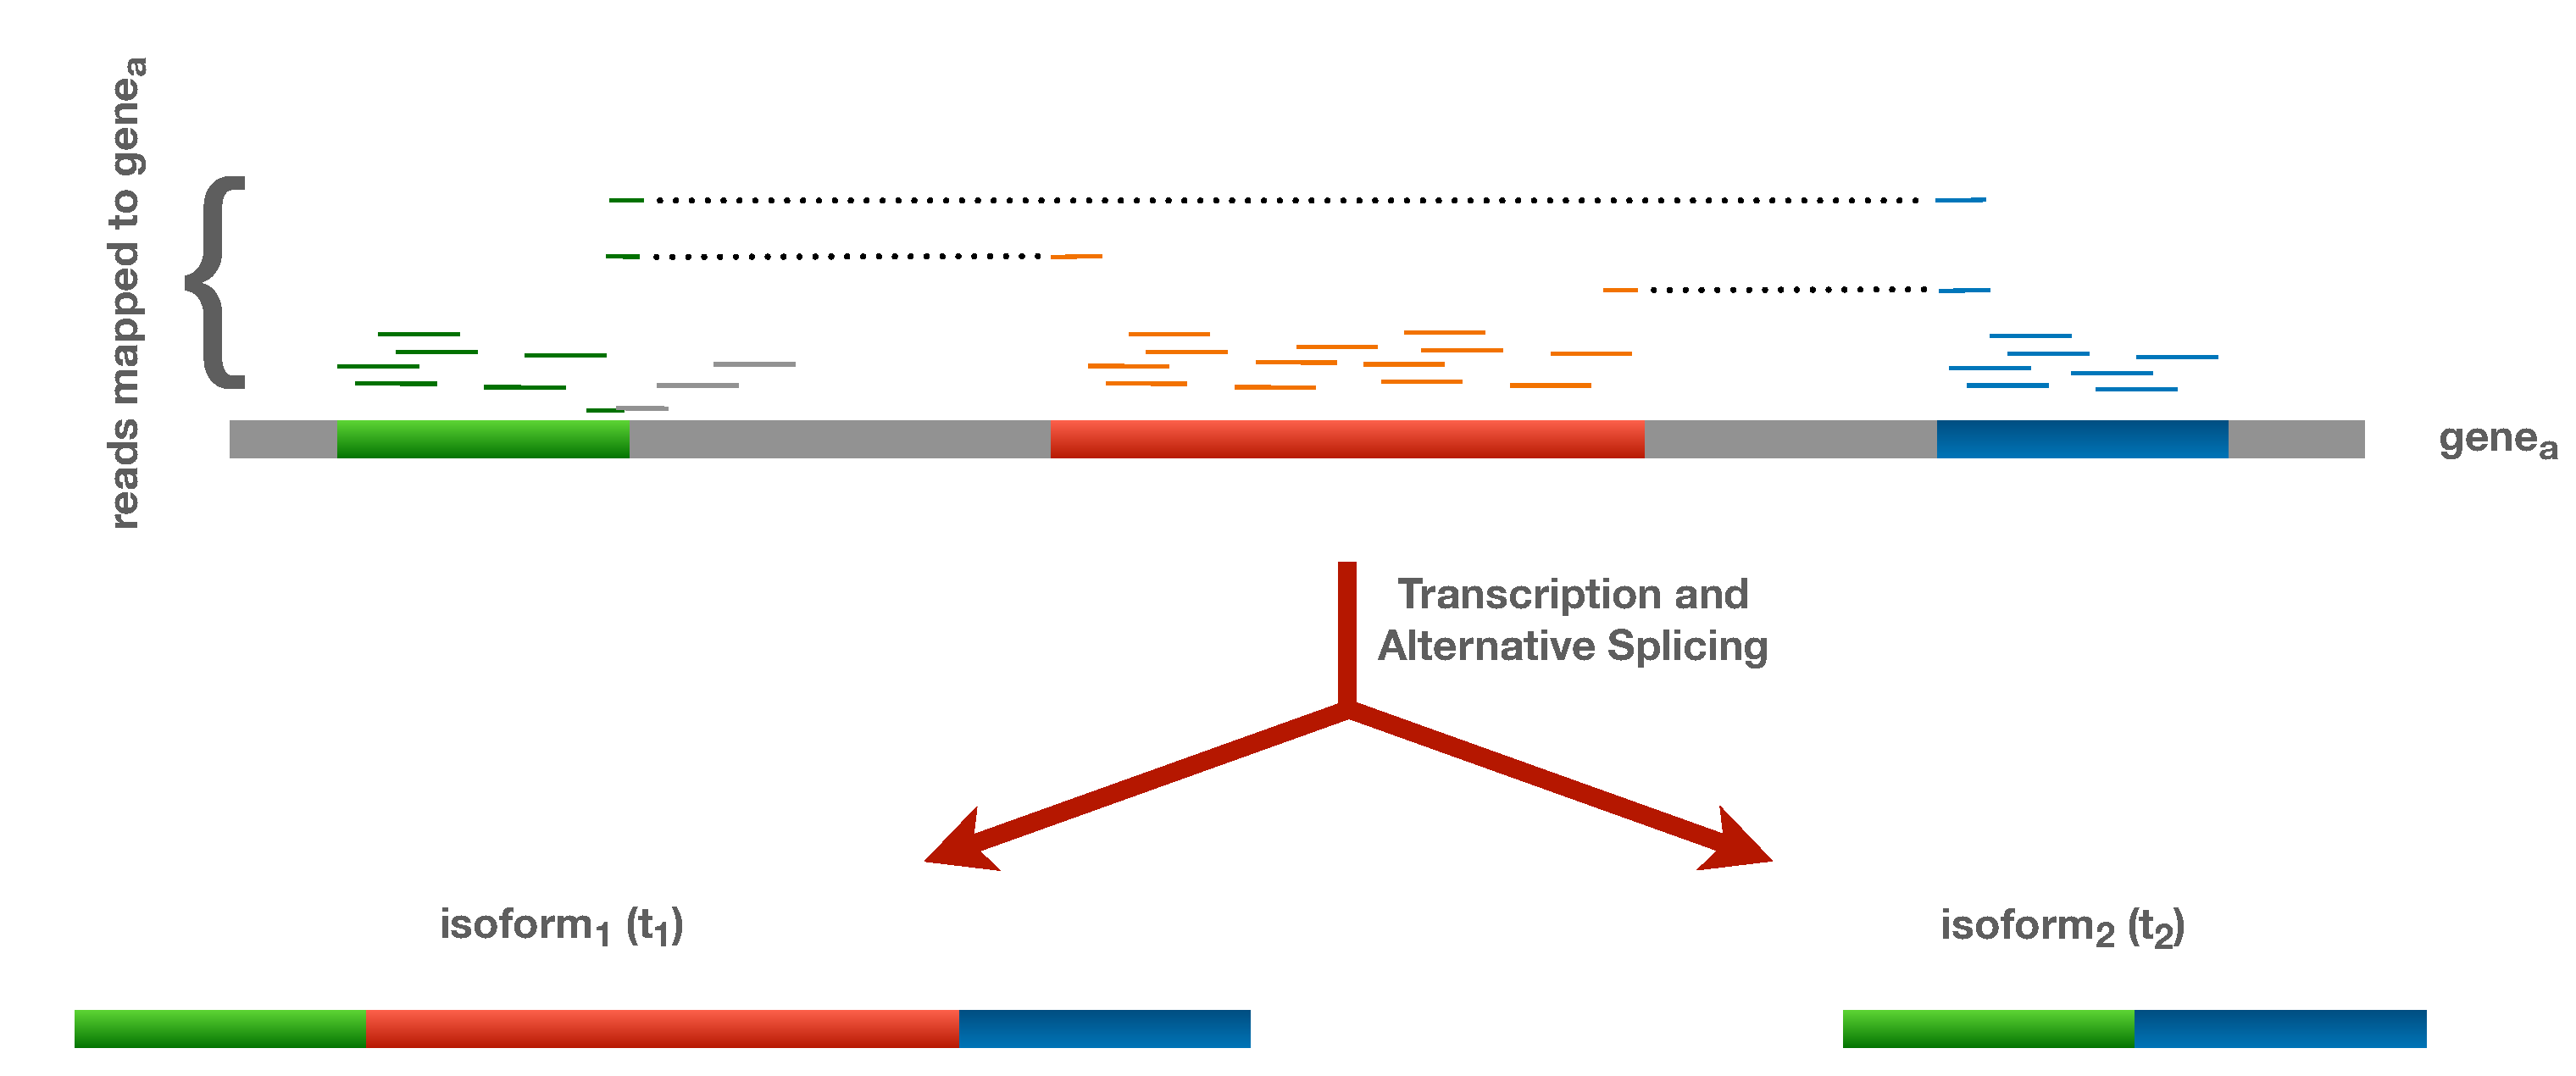
\includegraphics[width=0.95\columnwidth]{Figures/intro/alt-splice.pdf}
 \caption[Alternative splicing of genes]{An example of splicing events in 
 the gene $gene_a$, resulting in two transcripts $t_1$ and $t_2$. According 
 to sequence similarities the RNA-seq reads might be mapped to single or 
 multiple isoforms.}
  \label{fig:altsplice}
\end{figure}

In the following sections of this chapter I review the existing tools which 
are widely used for alignment (computing the compatibility of the reads to 
the reference sequences) and quantification (estimating the expression ratio 
of the isoforms) of RNA-seq samples. Both of these steps greatly affect the 
accuracy of the downstream analysis in RNA-seq 
pipelines~\citep{srivastava2019alignment}. In chapter 2, 
I present a fast mapping technique called \sla which is built 
alongside \qm to achieve a higher sensitivity which results in more 
accurate abundance estimates. Chapter 2 also introduces a new tool for 
computing alignment of DNA-seq and RNA-seq reads to known reference sequences. 
In chapter 3, an improved factorization of the quantification likelihood 
function is presented which  maintains a high fidelity to the underlying 
data and will result in higher confidence for more fine grained analysis 
of transcripts. 
% In chapter 4 the future work for my PhD research will be 
% proposed which involves projects for improving the RNA-seq quantification 
% accuracy and utilizing the equivalence classes for downstream analysis of 
% single cell samples. 
% In chapter 4, we briefly discuss performing further analysis with our 
% proposed methods, such as achieving more robust estimates by using different 
%optimization techniques.

\section{Mapping RNA-seq reads to a known transcriptome}

Alignment is a crucial and expensive computations step in an RNA-seq analysis 
pipeline. The main goal of this step is to find, for each read, the region on 
the reference genome (or transcriptome) from which it is originally fragmented. 
The length of the short RNA-seq reads is usually between 100 and 200 bases, 
while the latest human genome sequence is about three billion bases. The goal, 
for each read, is  to find a substring in the reference sequences which best 
matches the read. Often it is not possible to find an exact match for a read 
because of the variations present in the samples with respect to the reference 
sequences. The variations are divided into two main types, variations introduced 
by technical errors or the biological variations existing in each new sample. 
Therefore, the alignment procedure most of the time results in an inexact 
match for each read rather than a region which exactly matches the read. 
In order to find the most compatible reginos in the reference sequences to 
each read, we should define the compatibility of two sequences. The compatibility 
is measured by the number of edits required to convert one sequence to the 
other one. Different types of edits are considered which are substitution, 
insertion and deletion. The penalties assigned to each type of edit might be 
different and can be usually configured in most of the aligners. The sum of 
all the penalties is considered to be the edit distance between two sequences.
Therefore, we can define the alignment problem as finding the region on the 
reference with the minimum edit distance to each read. This can be achieved 
by classical algorithms such as Smith Waterman~\citep{smith1981identification} 
in $O(n*m)$ time and $O(n*m)$ space, where n and m are the length of the 
reference sequence and the read sequence respectively. This solution becomes 
super expensive when the length of reference sequences and the number read 
sequences are very large which is the common case in the RNA and DNA sequences. 
Therefore, a number of additional solutions proposed to accelerate this procedure 
while maintaining the accuracy of this approach. In the following sections, 
some of the main common approaches will be discussed briefly.

\subsection{The main approaches for computing read alignments}
One of the most common approaches for accelerating the alignment problem is 
“seed and extend”. The seeds are supposed to reduce the search space for the 
alignment problem into smaller regions that are most likely to include a 
reasonable alignment for the queried read rather than comparing each read 
sequence to all the reference sequences. Seeds are often shorter than the 
reads and represent an exact match from a substring in the read to some 
region in reference. The seeds are later extended into full alignments for 
the read by computing the full alignment of the reads to the regions 
identified by each read.

Finding the seeds requires the pre-processing of the reference sequences 
which is called the indexing step. Different indexing strategies are used 
in different aligners which have various space and time requirements. There 
are two main types of indices, full-text indices and hash-based indices. 
The full-text indices are often smaller in size, and a sequence of any different 
size can be queried in them, while the hash based indices take more space and 
only accept queries with a fixed size. The main benefit of the hash based indices 
are their speed compared to the full text indices. Full text indices are used in 
popular RNA-seq aligners such as Bowtie~\citep{bowtie}, Bowtie2~\citep{bowtie2}, 
BWA~\citep{bwamem} and STAR \citep{Dobin2013Star}. It is worth noting that STAR’s 
index employs a hybrid approach of both full text and hash based indices which 
results in being faster at the expense of larger memory requirements. 
Other aligners such as deBGA~\citep{debga}, Minimap2~\citep{minimap2}, are based 
on hash based indices and often use exact k-mer searches as the first step of 
the alignment step to find the seeds. K-mers of each read are all the substrings 
of length k in the read sequence. Querying a k-mer into the index results in 
finding all the locations on the reference sequences where the k-mer exists.

FM-index and Suffix Array are two closely related full text indices. The suffix 
Array (SA) of a string S with the length n is defined by the sorted order of all 
suffixes of string S concatenated with a terminal character which is 
lexicographically smaller than all other characters in the alphabet. 
Adding the terminal character ($\$$) ensures that no suffix is the prefix of any 
other suffix in S. In practice, the suffix array stores only the indices 
corresponding to each suffix in an array. If pattern p exist in the string S, 
then, it will be a prefix of some suffix in S. Lexicographically sorting the 
suffixes in SA, provides this property that all suffixes which include some 
pattern p as their prefix, will appear in consecutive rows in the SA. Therefore, 
to query a pattern in S, it suffices to find an interval [a,b) in the SA which 
are all the suffixes that include p as their prefix. Each pattern can be searched 
in the SA by a binary search, which takes O(log(|S|)x|p|). The search process can 
be enhanced by keeping some extra information like the longest common prefix 
lengths (LCP) for some pair of suffixes, as a result the query time will be 
O(log|S|+|p|) instead. STAR is one of the most popular aligners which use the 
Suffix Array to index the reference sequences. [cite] STAR uses some hash tables 
for accelerating the search process as well which comes at the cost of increasing 
the index size.

FM-Index is another full text index which consists of some auxiliary 
data structures alongside the Burrows Wheeler Transform (BWT) of the reference 
string S. BWT(S) is closely related to the Suffix Array. To enable efficient 
search for every pattern using BWT, the LF mapping property in the BWT is 
utilized with the help of storing the occurrence information of every character 
in the BWT. Using the succinct data structures, this can be stored in O(|S|) 
space. One other useful characteristic of the BWT is that it tends to put 
repetitions of each character next two each other, this doesn’t mean that all 
repetitions are put next to each other, but it is common to find longer 
substrings of A or any other character in the BWT of a sequence compared to the original sequence. This property of the BWT makes it more compressible compared to the original sequence which results in smaller index size. Bowtie, Bowtie2, and BWA are some of the popular aligners which index the reference sequences with a FM-Index.

The other main type of indices used for finding the alignment of a query in a 
large set of reference sequences are hash based indices. Hash based indices use 
substrings of a fixed size from the reference sequence to search each new query. 
The substrings of length k from the reference sequences are called k-mers. 
K-merss constitute the keys in the hash based indices. Hash based indices store 
the location where each k-mer occurs in the reference sequences. During the 
query time, we are able to extract all the k-mers from each read and query 
those e in the set of keys of the hash based index. The index will then 
retrieve all the positions each k-mer occurs in the reference which will 
later play the role of the seeds for the seed and extend procedure. It is 
important to note that queries of length smaller than k cannot be made into 
these hash based indices, so, one drawback of these types of indices is in 
order t o find a seed for the query  in the reference, there needs to be at 
least one substring of length k in the read which match the reference sequences 
without any edit distance. Therefore, the length of k should be carefully 
selected based on the error rate of the sequencing technology, so that with high 
probability at least one match from each read is found on the reference, if the 
read is actually originating from a position on the reference sequences.

\begin{figure}
 \centering
 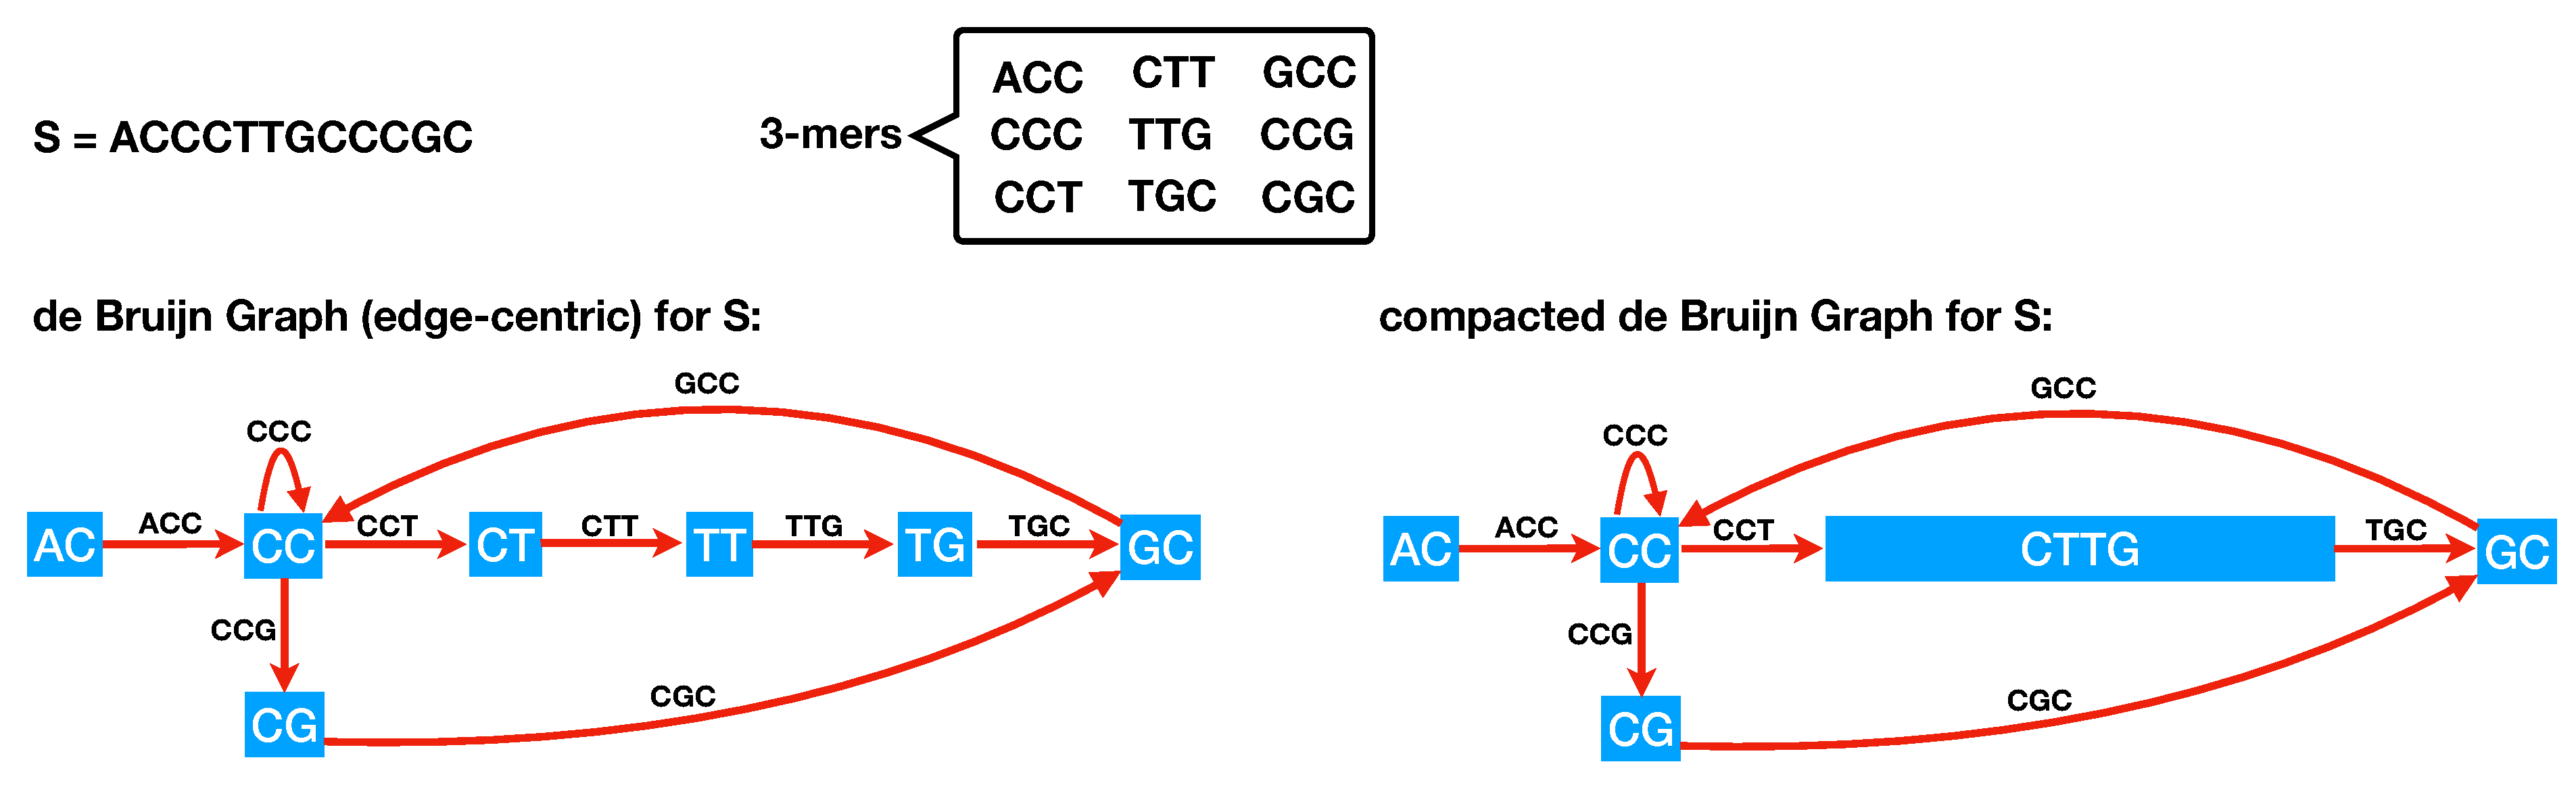
\includegraphics[width=0.95\columnwidth]{Figures/intro/deBruijnGraph.pdf}
 \caption[The edge-centric \dbg]{The edge-centric \dbg and the \cdbg for the 
 sequence S. There are 9 3-mers in this sequence which correspond to the edges 
 in the \dbg. 2-mers form the nodes of the \dbg. 3 nodes (CT, TT and TG) are 
 combined together in the \cdbg since they are on a non-branching path of the 
 \dbg.}
  \label{fig:dbg}
\end{figure}

Another approach for indexing all the \kmers of a set reference sequence is to 
build the \dbg. Each \kmer forms an edge in the de Bruijn graph between the 
prefix and suffix k-1 mers which it consists of. In the~\cref{fig:dbg}, a \dbg 
is shown which is built from the sequence S = “ACCCTTGCCCGC” and the k 
equal to 3. One main property in the de Bruijn graph is that every k-mer 
appears exactly once in the graph. This property helps to reduce the redundancy 
of repeats which usually exist in the DNA and RNA sequences. The compacted 
de Bruijn graph is built after compacting the non branching paths from the 
original de Bruijn graph, as shown in the~\cref{fig:dbg}. The length of the 
nodes in the compacted de Bruijn graph might be larger than k-1, but still 
each k-mer appears at most once in the graph (either as an edge or as a 
substring in one node). If the de Bruijn graph is built from multiple 
sequences (e.g., the set of human transcripts, or a collection of microbial 
genomes), one is interested to know in which reference sequences each k-mer 
appears. A k-mer might appear in multiple reference sequences due to shared 
exons in transcripts, or sequence similarities in different strains of some 
species.

A colored \dbg stores this data for each \kmer (edge) of the graph as the color 
information. For example, in the case of the transcriptome, each color represents 
the set of transcripts in which the \kmer corresponding to that edge exists. 
\Kmers appearing in the same set of transcripts (e.g., due to shared exons) 
will have the same colors. A contig in the \cdbg is a non branching path in 
the graph, and if the edges are colored, not all the k-mers in a contig might 
have the same color.
If all the \kmers that are part of a non branching path also have the same color 
set assigned, those \kmers can be combined together and form a unitig in the 
\ccdbg.

Pufferfish~\citep{pufferfish} is a space and time efficient index built on 
top of the compacted colored de Bruijn graph. So, it can be used to perform 
efficient k-mer queries from each read sequence to large transcriptomic or 
genomic references. In the second chapter of this manuscript, we introduce 
Puffaligner which uses the Pufferfish index to query k-mers from the short 
RNA-seq reads to compute read alignments through the seed and extend strategy.

\subsection{Alignment Free Approaches for Mappings reads}\label{int:qm}
Exploiting the methods of abundance estimation for RNA seq reads revealed the 
fact that although alignment is very useful for finding the candidate transcripts 
to which reads map, the full alignment information (The exact details of all the 
gaps and mismatches) are unnecessary for performing quantification. In fact the 
position, orientation and length of the matching fragment on each transcript is 
adequate for achieving accurate estimates. Therefore, lightweight methods were 
developed to avoid performing full alignments upstream of the quantification. 
These methods typically build an index over the reference sequence (similar to 
the FM index in alignment tools). Then, in the quantification step, the reads 
are mapped to the reference on the fly, rapidly, using the built-in index. 
Therefore, the memory peak footprint of such methods is bounded by the reference 
size and complexity and scales well as the number of reads increases. Note that 
for performing quantification over multiple samples to the same reference, the 
index needs to be built only once.

The first lightweight algorithm for mapping reads to reference transcripts was 
introduced in \sailfish \citep{Patro2014Sailfish}. \sailfish is an alignment-free 
quantification tool which builds an index over all subsequences of size k from the 
reference, called \kmers. The \sailfish index consists of a perfect hash function 
mapping each \kmer in the reference to a unique integer, an array indicating the 
counts of each \kmer, an index mapping each \kmer to the set of transcripts 
in which it appears, and another index mapping each transcript to the multiset 
of \kmers it contains. In the quantification step, \sailfish explores all the 
\kmers the read contains and keeps the count for the ones appearing in the 
reference. So instead of mapping the whole reads, \sailfish only maps the \kmers, 
and uses their count for each transcript as evidence for the relative expression 
of the transcripts. Although \sailfish's approach is 30 times faster than fastest 
quantification tools which perform alignment upstream of quantification, 
it suffers from increased ambiguity of a large rate of multi mapping \kmers, 
which sometimes reduces the accuracy of abundance estimation. The smaller k size 
causes a higher multi mapping rate, while the larger size of the k results in 
less robustness to sequencing errors because each \kmer is mapped with no error 
using the perfect hash function.

The idea of mapping \kmers instead of the whole reads to reference transcriptome 
introduces a huge improvement in the speed of quantification tools. However, 
it is sub-optimal to only consider occurrence of subsequences of size k as 
evidence of expression while the observed data is of larger length. Hence, 
the developers of \sailfish introduced a new idea for mapping the whole reads 
using the perfect hash function of \kmers by benefiting from the suffix array 
data structure. The new mapping approach is called \Qm \citep{Srivastava2016rapmap} 
and is utilized in the newer version of \sailfish software and also in the new 
quantification tool called \salmon \citep{Patro2017Salmon}. 

The suffix array of a sequence is a sorted array of all of the sequence's suffixes. 
Therefore, all suffixes starting with the same prefix are located in adjacent 
positions of the suffix array. Note that only the position of the occurrence of 
suffixes in $T$ are stored in the suffix array. The number of elements of the 
array is equal to the length of the sequence and there is a one-to-one mapping 
from each row of the suffix array to a character in the BWT of the sequence. We 
can also introduce suffix array intervals similar to intervals of the 
Burrows Wheeler transform. In the \qm index the suffix array $SA(T)$ is built from 
reference transcriptome $T$. Therefore, each row in the $SA$ starts at a unique 
transcript of the transcriptome. There is a hash function $I(k_i)=[b,c)$ from 
each \kmer $k_i$ in $T$ to a suffix array interval from row $b$ until row $c$; 
all rows that contain $k_i$ as a prefix. For mapping each read, the \kmers, $k_i$ 
of the read (existing in the hash table) are hashed to find SA intervals. It is 
often possible to extend a match between the query and a subset of rows of the SA 
interval. The \qm algorithm attempts to find the longest subsequence of the query 
starting with the $k_i$ as a prefix in the interval (also called maximum mappable 
prefix of $k_i$ ($MMP_i$) \citep{Dobin2013Star}) with a binary search, as the SA 
is sorted lexicographically.
\Qm retrieves a set of transcripts for each \kmer, the transcripts appearing 
in all sets are reported as mapping candidates for the read. The reverse 
complement of the read is also mapped and the sequence (either forward or 
reverse complement) with the higher number of matching \kmers determines the 
mapping orientation. For paired end reads, the other end of the read is also 
quasi-mapped to the reference. Then, transcripts appearing as candidates for 
both ends of the reads are reported as the mapping possibilities for the paired 
end reads.

It has been demonstrated that \qm finds very high quality mappings which result 
in highly-accurate abundance estimations. However, there are different aspects of 
the algorithm which can be modified in order to retrieve mappings with higher 
specificity and sensitivity. In fact, this idea is presented in chapter 2 as 
\sla. \Qm extends the \kmer matches by the MMP length in order to find legitimate 
matches for queries. However, if an extension is not possible and no other \kmer 
match exists in the read, \qm may report all transcripts of the interval as the 
mapping candidates for the read. These low quality matches introduce a number 
of spurious mappings. A filtering process shall be introduced in order to filter 
the spurious hits in this case. Other than suffering from spurious mappings \qm 
could also miss true mappings of the read in rare cases where errors are 
positioned adversarially on the read. An obvious case of losing the true mapping 
is if a read contains no subsequence of size $k$ from the true transcript. In 
another case, the true mapping of the read might be lost from the SA interval 
by performing MMP extension, if a longer exact match of the read to the interval 
masks the match to the row with true location. The hits in the reverse complement 
of the read are only considered if there are less number of hits in forward strand 
compared to reverse complement. Therefore, spurious mappings in the forward strand 
might mask the true hit in the reverse complement. For some reads, multiple 
positions might be found on the same transcript where the read maps. \Qm 
greedily considers the left most one as the true mapping while that might 
not be the best possible matching of the read to that transcript. To address 
these challenges in \qm, \sla is introduced as a new lightweight approach to 
achieve both higher sensitivity and specificity than \qm.

A similar approach to \qm is employed in \kallisto \citep{Bray2016Kallisto} 
called \pa. \kallisto index consists of a colored deBruijn graph from reference 
where nodes are \kmers and each node receives the colors of transcripts in which 
it appears. The contigs in the graph are formed from the linear stretches of the 
nodes (\kmers) with identical sets of colors. \Kallisto also maintains a hash 
table mapping each \kmer to the contig it is contained in and the \kmer's position 
in the contig. Using this index, the reads' \kmers are mapped to contigs. Since 
all the \kmers appearing in the same contig receive the same set of colors, and 
therefore the same transcripts, the rest of the \kmers in the contig can be 
skipped for mapping, similar to the idea of NIP skipping in \qm.

\section{Abundance estimation of the transcriptome}
In this section, we formalize the problem of abundance estimation with RNA-seq 
reads according to the model laid out by~\citet{Li2010RSEM}. There are $M$ 
transcript types in transcriptome $T$, $t_1, t_2, ..., t_M$. In a given sample 
there are $c_i$ copies of transcript type $t_{i}$, which are not observed directly.

\subsection{The generative model of a sequencing experiment}
\label{subsec:likelihood}

The generative model of RNA-seq experiments states that the number of fragments 
sequenced from $i^{th}$ transcript type is proportional to the total number of 
sequenceable nucleotides belonging to transcripts of type $t_i$. If the length 
of the $i^{th}$ transcript is given by $l_i$, assuming all the reads have the 
size $l_r$, we can define effective length, $\tilde{l}_i = l_i-l_r+1$ which is 
all possible start positions on transcript $t_i$ for sequencing a read of size 
$l_r$. The portion of sequenceable nucleotides of transcript type $t_i$ is 
$ \eta_i = \frac{c_il_i}{\sum_{j}{c_jl_j}}$ and $\alpha_i \propto \eta_i$, 
where $\alpha_i$ is the number of fragments drawn from transcripts of type $t_i$.

If $\fragments$ with $|\fragments|=N$, is the set of sequenced fragments, 
assuming independence for drawing each fragment, the likelihood of the underlying 
transcript abundances, $\theta$, can be written as:

\begin{equation}
  \likelihood{\bm{\theta}; \fragments} = \prod_{f_i \in \fragments}  
  \sum_{j=1}^{M} \Pr\left(t_i \mid \bm{\theta}\right) 
  \Pr\left( f_i \mid t_j \right).
  \label{eqn:likelihood_fm1}
\end{equation}

The conditional probability of drawing a particular fragment $f_i$, given 
transcript $t_j$, $\Pr{(f_i|t_j)}$, is particularly critical for reaching 
accurate estimates and is derived from mapping information.  This term encodes, 
given parameters of the model and experiment, how likely it is to observe a 
specific fragment $f_i$ arise from transcript $t_j$.
Many terms can be included in such a conditional probability, 
some common terms include:

\begin{equation}
  \Pr\left( \fraglen{i} \mid f_i, t_j\right) = \frac{\Pr_D\left( \fraglen{i}\right)}{\sum_{k=1}^{\tilde{l}_j} \Pr_D\left( k \right)},
  \label{eqn:pr_len1}
\end{equation}

the probability of observing a mapping of implied length $\fraglen{i}$ 
for $\frag{i}$ given that it derives from $\txp{j}$, where $\Pr_D\left(k\right)$ 
is the probability of observing a fragment of length $k$ under the empirical 
fragment length distribution $D$;

\begin{equation}
  \Pr\left( p_i \mid \fraglen{i}, f_i, t_j\right) = \frac{1}{l_j - \fraglen{i} + 1},
  \label{eqn:pr_start1}
\end{equation}

the probability of a observing a mapping starting at position $p_i$ for 
fragment $\frag{i}$ given that it has implied length $\fraglen{i}$ and is 
derived from $\txp{j}$;

\begin{equation}
  \Pr\left( o_i \mid \frag{i}, \txp{j} \right)  = 
      \begin{cases}
    \begin{cases}
      0.5 
    \end{cases}
    & \text{if unstranded}\\
    \begin{cases}
      1.0 & \text{if compatible orientation} \\
      \epsilon & \text{if incompatible orientation}
    \end{cases} &\text{if strand-specific}
      \end{cases},
  \label{eqn:orient1}
\end{equation}

the probability of observing a mapping with a specific orientation $o_j$ 
(i.e., forward or antisense) with respect to the underlying transcript for 
$\frag{j}$, given $\txp{i}$, $\epsilon$ (a user-defined constant), and knowledge of the underlying protocol, 
and

\begin{equation}
   \Prob{a_i}{\frag{i}, o_i, \fraglen{i}, p_i, \txp{j}},
  \label{eqn:align1}
\end{equation}

the probability of observing the particular alignment (e.g., \texttt{CIGAR}
string) $a_i$ for $\frag{i}$ given it is sampled from transcript $\txp{j}$, has
orientation $o_i$, implied length $\fraglen{i}$ and starts at position
$p_i$---such a probability is calculated from a model of alignments, like those 
presented in~\citep{Li2010RSEM,Roberts2013Express,Patro2017Salmon}.

In fact, one can conceive of many such general models of ``fragment-transcript
agreement''~\citep{Patro2017Salmon}. However, here we consider that 
$\Prob{f_j}{t_i}$ is simply the product of the conditional probabilities 
defined in~\Cref{eqn:pr_len1,eqn:pr_start1,eqn:orient1,eqn:align1}, appropriately 
normalized.


\subsection{Expectation-Maximization for optimizing the model parameters}
Exact inference from the likelihood function is intractable for the large 
scale of RNA seq data. Local optimization methods, like expectation 
maximization (EM), are often applied to fit the best parameters in the model. 
The parameters of the model indicate the rate of expression for each transcript 
in the underlying samples. The EM approach is employed by both alignment based 
tools such as \rsem \citep{Li2010RSEM}, \mmseq~\citep{Turro2011Haplotype}, 
\isoem~\citep{Nicolae2011Estimation} and also non-alignment based tools like 
\sailfish \citep{Patro2014Sailfish}, \salmon \citep{Patro2017Salmon} and 
\kallisto \citep{Bray2016Kallisto}. 

\begin{algorithm}[H]
\SetAlgoLined
\KwData{transcriptome $T$, fragment set $\fragments$,conditional properties 
$ \Pr{(f_i|t_j)}$ for fragment transcript pairs}
 \KwResult{$\theta$, relative abundance of transcripts}
  uniform initialization\;
 \While{not converged}{
 \For{$t_i \in T$}{
  $\alpha_i = 0$,  $\theta_i = \frac{1}{|T|}$ 
 }
\textcolor{blue}{E-step:} \\

\For{$f_i \in \fragments$}{
 $sum = \sum_{t_k \in T}{\theta_k \times  \Pr{(f_i|t_k)}}$\\
 \For{$t_j \in T$}{
    $\alpha_j += \frac{\theta_j \times  \Pr{(f_i|t_j)}}{sum}$
 }
}
\textcolor{blue}{M-step:} \\
$sum = \sum_{t_k \in T}{\frac{\alpha_k}{\tilde{l_k}}}$\\
 \For{$t_i \in T$}{
$ \theta_i = \frac{\alpha_i/\tilde{l_i}}{sum}$
} 
}
\caption{Overview of the EM algorithm for optimizing the generative model}
 \label{EM-alg}
\end{algorithm}

The overview of the EM algorithm for optimizing~\cref{eqn:likelihood_fm1} is 
displayed in algorithm \ref{EM-alg}. In the E-step, the expected number of 
fragments sequenced from each transcript type in the sample is calculated. 
Using these expectations, alongside effective lengths the prior probability of 
observing each transcript type is obtained in the M-step. This iterative process 
is repeated until the convergence on $\theta$ values is reached. 

If a transcript $t_j$ is not present in the set of transcripts to which 
fragment $f_i$ is mapped, the  value of $\Pr{(f_i|t_j)}$ is equal to zero. 
The EM updates can benefit from the sparsity of $\Pr{(f_i|t_j)}$ matrix by 
only performing updates in the E-step for the set of transcripts that $f_i$ maps 
to instead of the whole set of transcripts. Hence, if $\Omega{(f_i)}$ is the set 
of compatible transcripts with read $f_i$, in algorithm~\ref{EM-alg}, the line 8 
shall be modified to : 
$sum = \sum_{t_k \in \Omega{(f_i)}}{\theta_k \times  \Pr{(f_i|t_k)}}$\  
and the loop iteration in line 9 to :   $t_j \in \Omega{(f_i)}$.

\subsection{Factorizations of the likelihood function}\label{int:fact}

Each iteration of the EM algorithm updates the $\alpha$ values for each fragment 
independently. Although each update cost has collapsed considerably by benefiting 
from the sparsity of mapping matrix, the number of EM updates still scales with 
the number of fragments (and alignments). Sequence similarities in reads shall be 
utilized for factorizing the likelihood function, which results in bounding the 
number of updates as the number of fragments grows.
 
If a set of fragments, $F'$, exactly map to the same set of transcripts, $T'$, 
with the same conditional probabilities (meaning that for each pair 
$f_i,f_j \in F'$, $\Omega{(f_i)}=\Omega{(f_j)}=T'$ and the equation 
$\Pr{(f_i|t_k)}=\Pr{(f_j|t_k)}$ holds for all $t_k \in T'$), then all 
fragments in $F'$ are exactly equivalent, and they result in the same update rule 
in the EM iterations. Hence, they can be grouped together to apply the update once 
for all such fragments. This factorization, which is introduced by 
\isoem \citep{isoem}, maintains full fidelity to information regarding fragment 
mappings to transcripts because all fragments in a group are identical.

A more popular approach for factorizing the likelihood is employed by 
\mmseq \citep{Turro2011Haplotype} and also later in alignment-free tools 
like \sailfish \citep{Patro2014Sailfish}, \salmon \citep{Patro2017Salmon} 
and \kallisto \citep{Bray2016Kallisto}. \mmseq introduced a notion of fragment 
equivalence classes, which treats as equivalent any fragments that map to the 
same set of transcripts. Unlike \isoem, the equivalence notion does not depend 
on the values of conditional probabilities.  According to this definition, every 
set of fragments like $\Frags^q$ such that for all 
$f_i,f_j \in \Frags^q$, $\Omega{(f_i)}=\Omega{(f_j)}=\Omega{(\Frags^q)}$, 
form an equivalence class with the label $\Omega{(\Frags^q)}$. 
Define $N^q=|\Frags^q|$ to be the number of fragments in class $\Frags^q$. 
Then, the likelihood function based on these equivalence classes, can be 
approximated as:

\begin{equation}
    \likelihood{\bm{\theta}; \Frags} \approx 
        \prod_{\eqclass{q} \in \eqclasses}
        \left(\sum_{\langle i, t_i \rangle \in \mapset{\eqclass{q}}} 
        \Prob{\txp{i}}{\bm{\theta}} 
        \cdot \Prob{f}{\eqclass{q},\txp{i}} \right)^{\eqsize{q}},
\label{eqn:likelihood_fact}
\end{equation}

where $\eqclasses$ is the set of all equivalence classes, and
$\Prob{f}{\eqclass{q},\txp{i}}$ is the probability of generating a fragment $f$
given that it comes from equivalence class $\eqclass{q}$ and transcript
$\txp{i}$. The key to the efficiency of likelihood evaluation (or optimization)
under this factorization, is that the probability $\Prob{f}{\eqclass{q},\txp{i}}$ 
is assumed to be identical for each of the $\eqsize{q}$
fragments in each equivalence class $\eqclass{q}$---hence, we do not
subscript $f$ in~\cref{eqn:likelihood_fact}. This allows one to replace the
product over all fragments $f_j$ in full model (\cref{eqn:likelihood_fm1}) with 
a product over all equivalence classes in \cref{eqn:likelihood_fact}. 
The approximation, of course, stems from the fact that, under the full model, 
a fragment $\frag{j}$ may have a probability 
$\Prob{\frag{j}}{\txp{i}}$ that is arbitrarily different
from $\Prob{f}{\eqclass{q},\txp{i}}$. Moreover, the most common approximations,
like those adopted in \mmseq, \sailfish, and \kallisto consider this
probability to be fixed and essentially independent of any fragment-level
information (e.g., it is set to one divided by the effective
length of $\txp{i}$).

After applying any factorization which groups a set of fragments together 
in equivalence classes $\Frags^q$, the fragments in the EM iteration can 
be substituted with equivalence classes (groups) and each update would 
increase the $\alpha$ values based on the number of fragments in each 
equivalence class. The modified version of the E step 
in algorithm \ref{EM-alg} is displayed in algorithm \ref{EM-alg2}.

\begin{algorithm}[H]
\textcolor{blue}{E-step:} \\
\For{$\Frags^q \in \eqclasses$}{
 $sum = \sum_{t_k \in \Omega{(\Frags^q)}}{\theta_k \times  \Pr{(f|\Frags^q,t_k)}}$
 \\
 \For{$t_j \in \Omega{(\Frags^q)}$}{
    $\alpha_j += \frac{\theta_k \times  \Pr{(f|\Frags^q,t_k)}}{sum}$
 }
}
\caption{Modified E step after employing factorization}
 \label{EM-alg2}
\end{algorithm}


\subsection{Online EM for optimizing the likelihood function}

The conditional probability values are stored in memory during the EM iterations 
in order to avoid expensive I/O operations and re-computation in each EM round. 
If no factorization is used, for each existing mapping pair $f_i$ and $t_j$, 
a value is stored. This makes the memory requirement scale with the number of 
mappings. \express \citep{Roberts2013Express} attempts to bound the memory 
requirement by benefiting from an online-EM algorithm rather than a batch-EM. 
An online-EM consists of a single iteration over all fragments in the sample, 
updating $\alpha$ values once for each fragment. Fragments are not stored in 
memory after being observed, which makes \express's memory requirement 
independent of the number of fragments in the sample. The large number of 
fragments in RNA-seq samples lets \express often achieve high quality abundance 
estimates with a single run over the data. \express requires the output 
of an alignment tool for mapping reads to transcripts to run the online phase. 
Again, here, the mapping information shall limit the number of updates performed 
for each fragment. 

\express applies a modified version of online updates which prevents the 
algorithm from performing updates for each transcript in each iteration. 
The online update rules for each fragments are:
\begin{equation}
\alpha^{i+1} = \alpha^{i}+m_i\tilde{\tau}^i,
\label{eqn:online1}
\end{equation}
where:
\begin{equation}
\tilde{\tau}^i_t =\Pr{(T=t|F=f_i)},
\label{eqn:online2}
\end{equation}
and
\begin{equation}
m_{i+1} = m_i \times \frac{\gamma_{i+1}}{1-\gamma_i} \times \frac{1}{\gamma_i},
\label{eqn:online3}
\end{equation}

$\alpha^i$ is the optimized value after observing the first i fragments. 
Bayes' rule can be applied to obtain the probability in \cref{eqn:online2} 
from the conditional probabilities. The value $m_i$ is called forgetting 
mass and depends on the forgetting factor $\gamma_i$. The $\gamma$ values 
are set as $\gamma_i=\frac{1}{i^c}$ where $0.5<c<1.0$. After observing 
all $N$, fragments the relative counts of fragments from each transcript type 
can be obtained from the vector $\alpha^N$.

\subsection{Dual phase optimization}
The inference algorithm in \salmon \citep{Patro2017Salmon} consists of two phases. 
First, \salmon runs an online EM optimization to obtain high quality primary 
estimates of abundances. In this phase, \salmon is able to achieve a good 
estimation of fragment length distribution by examining many fragments as 
they are streamed in the online EM. Therefore \salmon can derive good estimates 
of conditional probabilities using the fragment length distribution and other 
information provided with mappings. The equivalence classes over sets of 
fragments are also created in the online phase. \salmon introduces the notion 
of rich equivalence classes by assigning a single scalar to each transcript in 
an equivalence class, by averaging the conditional probabilities of all fragments 
in the class to the transcript. This value is equal to $\frac{1}{|\Omega{(F^q)}|}$ 
in non-rich equivalence classes. 

\salmon uses the estimates obtained in the online phase as a starting point 
for performing a batch EM algorithm in the second phase. This two-phase 
optimization allows \salmon to rich very high quality estimates compared 
to other existing quantification tools. The online phase of the \salmon 
enables deriving a new factorization of the likelihood function to be 
optimized in the batch EM phase, which does not discard any necessary 
information for accurate abundance estimation. The details of this 
factorization is discussed in chapter 3.

\subsection{Metrics for evaluating quantification accuracy}
The formula for calculating the metrics used for evaluating the 
abundance estimation results in the manuscript are as follows. 
The metrics are Mean Absolute Relative Difference (MARD), Mean Absolute
Error (MAE), and Mean Squared Log Error (MSLE).

\begin{equation}
\begin{split}
    \text{MARD}(y, \hat{y}) = \frac{1}{n_{\text{refs}}} 
    \sum_{i=0}^{n_{\text{refs}}-1}
    {\frac{ \left| y_i - \hat{y}_i \right|}{y_i + \hat{y}_i}}. 
    \\
    \text{MAE}(y, \hat{y}) = \frac{1}{n_{\text{refs}}} 
    \sum_{i=0}^{n_{\text{refs}}-1} \left| y_i - \hat{y}_i \right|. 
    \\
    \text{MSE}(y, \hat{y}) = \frac{1}{n_\text{refs}} 
    \sum_{i=0}^{n_\text{refs} - 1} (y_i - \hat{y}_i)^2. 
    \\
\end{split}
\label{eq:metrics}
\vspace{-7mm}
\end{equation}

All of these metrics compute the difference of the estimated abundances 
with the truth. In addition to these metrics, we also evaluate the 
correlation between the estimations and truth by computing the 
Spearman correlation. Spearman correlation is computed using the 
pandas library~\citep{reback2020pandas} in Python.

\subsection{Inference of the Posterior Distribution of RNA-seq quantification}
Estimating the inference uncertainty of the RNA-seq quantification is one of the crucial
steps for many downstream analysis, e. g., finding the differentially expressed genes or 
transcripts, i. e., DE analysis. In fact, methods like Swish~\cite{zhu2019nonparametric}
directly use the inferential replicates created by RNA-seq quantification tools for finding
the DE genes with a higher precision compared to other approaches.

There are two main approaches for sampling the posterior distribution for estimating the 
uncertainty of quantification estimates; \gibbs and \boots. The \gibbs is a MCMC procedure
which walks through the space that the EM explores for finding the \mles of the \txps expressions.
At the end of each iteration of the \gibbs, the \txp expression vector could be identified
as a new inferential replicate for estimating the posterior distribution. To decrease between
replicate correlations, the sampling could take place after every fixed number of iterations which
is called the thinning factor for the sampling. Running the \gibbs procedure for long enough 
could reach to the convergance of the posterior estimate, this will be only reached only after
the Gibbs sampler has explored all the posterior samples. The number of iterations which is
required for \gibbs to converge usually depends on the properties of the sample, and as the number
of \txps in the sample increases the convergance usually takes longer.

% talk about bootstrap sampling
\boots is the other main approach for estimating the posterior distribution of the abundance
estimations in RNA-seq. The bootstrap procedure \cite{efron1979computers} is a widely-used 
and computationally straightforward procedure for calculating measures of accuracy of an 
estimator. It works by resampling (with replacement) from the observed data, and treating 
these as population samples. The procedure has been used in many contexts for non-parametric 
estimation. In RNA-seq, Computing the abundance estimation of all \boot sample leads to a 
estimating a posterior distribution for the abundances. 
